% ----------------------------------------------------
% Literature Review
% ----------------------------------------------------
\documentclass[class=report,11pt,crop=false]{standalone}
% Page geometry
\usepackage[a4paper,margin=20mm,top=25mm,bottom=25mm]{geometry}

% Font choice
\usepackage{lmodern}

% Use IEEE bibliography style
\bibliographystyle{IEEEtran}

% Line spacing
\usepackage{setspace}
\setstretch{1.20}

% Ensure UTF8 encoding
\usepackage[utf8]{inputenc}

% Language standard (not too important)
\usepackage[english]{babel}

% Skip a line in between paragraphs
\usepackage{parskip}

% For the creation of dummy text
\usepackage{blindtext}

% Math
\usepackage{amsmath}

% Header & Footer stuff
\usepackage{fancyhdr}
\pagestyle{fancy}
\fancyhead{}
\fancyhead[R]{\nouppercase{\rightmark}}
\fancyfoot{}
\fancyfoot[C]{\thepage}
\renewcommand{\headrulewidth}{0.0pt}
\renewcommand{\footrulewidth}{0.0pt}
\setlength{\headheight}{13.6pt}

% Epigraphs
\usepackage{epigraph}
\setlength\epigraphrule{0pt}
\setlength{\epigraphwidth}{0.65\textwidth}

% Colour
\usepackage{color}
\usepackage[usenames,dvipsnames]{xcolor}

% Hyperlinks & References
\usepackage{hyperref}
\definecolor{linkColour}{RGB}{77,71,179}
\hypersetup{
    colorlinks=true,
    linkcolor=linkColour,
    filecolor=linkColour,
    urlcolor=linkColour,
    citecolor=linkColour,
}
\urlstyle{same}

% Automatically correct front-side quotes
\usepackage[autostyle=false, style=ukenglish]{csquotes}
\MakeOuterQuote{"}

% Graphics
\usepackage{graphicx}
\graphicspath{{Images/}{../Images/}}
\usepackage{makecell}
\usepackage{transparent}

% SI units
\usepackage{siunitx}

% Microtype goodness
\usepackage{microtype}

% Listings
\usepackage[T1]{fontenc}
\usepackage{listings}
\usepackage[scaled=0.8]{DejaVuSansMono}

% Custom colours for listings
\definecolor{backgroundColour}{RGB}{250,250,250}
\definecolor{commentColour}{RGB}{73, 175, 102}
\definecolor{identifierColour}{RGB}{196, 19, 66}
\definecolor{stringColour}{RGB}{252, 156, 30}
\definecolor{keywordColour}{RGB}{50, 38, 224}
\definecolor{lineNumbersColour}{RGB}{127,127,127}
\lstset{
  language=Matlab,
  captionpos=b,
  aboveskip=15pt,belowskip=10pt,
  backgroundcolor=\color{backgroundColour},
  basicstyle=\ttfamily,%\footnotesize,        % the size of the fonts that are used for the code
  breakatwhitespace=false,         % sets if automatic breaks should only happen at whitespace
  breaklines=true,                 % sets automatic line breaking
  postbreak=\mbox{\textcolor{red}{$\hookrightarrow$}\space},
  commentstyle=\color{commentColour},    % comment style
  identifierstyle=\color{identifierColour},
  stringstyle=\color{stringColour},
   keywordstyle=\color{keywordColour},       % keyword style
  %escapeinside={\%*}{*)},          % if you want to add LaTeX within your code
  extendedchars=true,              % lets you use non-ASCII characters; for 8-bits encodings only, does not work with UTF-8
  frame=single,	                   % adds a frame around the code
  keepspaces=true,                 % keeps spaces in text, useful for keeping indentation of code (possibly needs columns=flexible)
  morekeywords={*,...},            % if you want to add more keywords to the set
  numbers=left,                    % where to put the line-numbers; possible values are (none, left, right)
  numbersep=5pt,                   % how far the line-numbers are from the code
  numberstyle=\tiny\color{lineNumbersColour}, % the style that is used for the line-numbers
  rulecolor=\color{black},         % if not set, the frame-color may be changed on line-breaks within not-black text (e.g. comments (green here))
  showspaces=false,                % show spaces everywhere adding particular underscores; it overrides 'showstringspaces'
  showstringspaces=false,          % underline spaces within strings only
  showtabs=false,                  % show tabs within strings adding particular underscores
  stepnumber=1,                    % the step between two line-numbers. If it's 1, each line will be numbered
  tabsize=2,	                   % sets default tabsize to 2 spaces
  %title=\lstname                   % show the filename of files included with \lstinputlisting; also try caption instead of title
}

% Caption stuff
\usepackage[hypcap=true, justification=centering]{caption}
\usepackage{subcaption}

% Glossary package
% \usepackage[acronym]{glossaries}
\usepackage{glossaries-extra}
\setabbreviationstyle[acronym]{long-short}

% For Proofs & Theorems
\usepackage{amsthm}

% Maths symbols
\usepackage{amssymb}
\usepackage{mathrsfs}
\usepackage{mathtools}

% For algorithms
\usepackage[]{algorithm2e}

% Spacing stuff
\setlength{\abovecaptionskip}{5pt plus 3pt minus 2pt}
\setlength{\belowcaptionskip}{5pt plus 3pt minus 2pt}
\setlength{\textfloatsep}{10pt plus 3pt minus 2pt}
\setlength{\intextsep}{15pt plus 3pt minus 2pt}

% For aligning footnotes at bottom of page, instead of hugging text
\usepackage[bottom]{footmisc}

% Add LoF, Bib, etc. to ToC
\usepackage[nottoc]{tocbibind}

% SI
\usepackage{siunitx}

% For removing some whitespace in Chapter headings etc
\usepackage{etoolbox}
\makeatletter
\patchcmd{\@makechapterhead}{\vspace*{50\p@}}{\vspace*{-10pt}}{}{}%
\patchcmd{\@makeschapterhead}{\vspace*{50\p@}}{\vspace*{-10pt}}{}{}%
\makeatother
\makenoidxglossaries
% --------------------------------------------------------------------
% Examples of creating a glossary
\newacronym{cw}{CW}{Continuous-Wave}
\newacronym{dsp}{DSP}{Digital Signal Processing}
\newacronym{em}{EM}{Electromagnetic}
\newacronym{fmcw}{FMCW}{Frequency Modulated Continuous Wave}
\newacronym{gui}{GUI}{Graphical User Interface}
\newacronym{rf}{RF}{Radio Frequency}
\newacronym{radar}{RADAR}{Radio Detection and Ranging}
\newacronym{pcb}{PCB}{Printed Circuit Board}
\newacronym{pc}{PC}{Personal Computer}
\newacronym{pri}{PRI}{Pulse Repetition Interval}
\newacronym{adc}{ADC}{Analogue-to-Digital Converter}
\newacronym{if}{IF}{Intermediate Frequency}
\newacronym{itu}{ITU}{International Telecommunications Union}
\newacronym{rcs}{RCS}{Radar Cross Section}
\newacronym{opamp}{Op Amp}{Operational Amplifier}
\newacronym{gbwp}{GBWP}{Gain Bandwidth Product}
\newacronym{dc}{DC}{Direct Current}
\newacronym{ac}{AC}{Alternating Current}
\newacronym{uct}{UCT}{University of Cape Town}
\newacronym{usb}{USB}{Universal Serial Bus}
\newacronym{stft}{STFT}{Short-Time Fourier Transform}
\newacronym{fft}{FFT}{Fast Fourier Transform}
\newacronym{dft}{DFT}{Discrete Fourier Transform}
\newacronym{dtft}{DTFT}{Discrete-Time Fourier Transform}
\newacronym{snr}{SNR}{Signal-to-Noise Ratio}
\newacronym{prf}{PRF}{Pulse Repetition Frequency}
\newacronym{isar}{ISAR}{Inverse Synthetic Aperture}
% include SUV (check experimentation table)
% --------------------------------------------------------------------

\begin{document}
\ifstandalone
\tableofcontents
\fi
% ----------------------------------------------------
\chapter{Literature Review \label{ch:literature}}
\vspace{-1cm}
% ----------------------------------------------------
This chapter gives a survey of existing literature related to ultrasonic radar and its applications in industry. A brief history of ultrasonic radar systems is explored and its past, current, and future applications are further included to provide a clearer picture of the benefits of using ultrasonic radar. Thereafter, some fundamental concepts of ultrasonic radar systems is surveyed before key differences between \gls{cw} radars and pulsed radars are provided to single out the advantages of using \gls{cw} radar over pulsed radar. An introduction to the use of the spectrogram for processing radar data is then provided to give context on the signal processing used in this project. Once this has been established, some factors that affect the performance of ultrasonic radar systems are mentioned to highlight how this project aims to reduce these limiting factors to increase the performance of the final demonstrator. Existing vehicle speed-estimation systems are provided along with Doppler concepts which are an integral part of this project. Finally, a critique on the literature is provided.
% Alternative sentence: Existing ultrasonic radar applications and vehicle speed-estimation systems are provided along with Doppler concepts which are an integral part of this project

\section{Brief History of Ultrasonic Radar Systems}
The history of ultrasonic \gls{radar} naturally begins as a history of \gls{radar} itself. With its lengthy developmental history, it would be difficult to attribute the creation of \gls{radar} to an individual or group, but a good starting point is the work conducted by Scottish mathematical physicist, James Maxwell. In 1865, Maxwell published his seminal work where the \emph{Maxwell's equations} were first demonstrated \cite{maxwell}. German physicist Heinrich Hertz, began performing experiments on electromagnetic radiation during the late 1880s, working to verify \emph{Maxwell's equations} which led to the his demonstration of the reflection of \gls{em} waves \cite{hertz, cichon}. 

In 1904, Christian H\"ulsmeyer, a German engineer, was issued a patent for a device he marketed as an anti-collision device for ships that used \gls{em} prinicples based on the work done by Hertz \cite{swords}. Although his device failed to arouse any interest, the need for long-range military bombers capable of carrying large loads increased in the early 1930s \cite{pomr, mitlecture}. Prior to World War II, other methods of ship and aircraft detection were used including the use of infrared sensors, but these methods proved to be ineffective. This quickly led to many countries experimenting with radar technology for military purposes; effectively many countries had operational radar military equipment at the start of World War II. Since then, much progress has been made on the development of radar technology for target detection, range measurement, and velocity calculation \cite{skolnik}. 

Although radar has been around for a while, ultrasonics had its beginning in 1794 when physiologist, Lazzaro Spallanzani, discovered the echolocation among bats \cite{tripathi}. Tripathi et al. in \cite{tripathi} note that the discovery of the piezoelectric effect by French physicist Pierre Curie and his brother Jacques Currie, provide the most notable breakthrough of ultrasonic technology. In 1917, Paul Langevine used high frequency based electrostatic sound transmitters and quartz resonators to detect submarines \cite{bok}. This use of sonar was the first practical application of piezoelectric technology and ultrasound developed during World War I. Ultrasonic technology was further developed over the years and was found useful during World War II, especially in its use for medical diagnosis as developed by the neurologist, Karl Dussik in 1942 \cite{dussik}. Since then, countries like Japan and the USA have played significant roles in the development of ultrasonic technology for medical use as further explored in \cite{tripathi}.

Today, ultrasonic technology has found its place in many applications, often being preferred due to its robustness, accuracy to detect a variety of materials and its fast operation. Some useful applications of ultrasonic radar technology are: trash-level monitoring to detect the level of waste in trash bins, vehicle detection systems for car washes like the ParkSonar-EZ produced by MaxBotix, and the MB8450 car detection sensor for drive-throughs also produced by MaxBotix. This technology is also used in smart farming for drone altitude adjustments for collision prevention when spraying crop and in automating assembly and handling in factories. More examples of ultrasonic radar applications are provided by Gillespie in \cite{gillespie}. Ultrasonic technology has been well-explored and developed over the years and is a competitive selection for its generally low-cost, high-performance, and scalable nature.

\section{Fundamentals of Ultrasonic Radar Systems}
Ultrasonic radar transmits \gls{em} waves towards a target detects the echoed signal using a respective transmitter and receiver. Unlike \gls{rf}-based systems, ultrasonic radars transmit sound waves \cite{pomr, tripathi}. To understand the workings of the ultrasonic radar, some fundamental principles must be laid down.

Range, $R$, is an important property of ultrasonic radar systems and is defined as the distance between the radar and the target object along the radar's line of sight \cite{pomr}. This concept is defined by Equation~\ref{eqn:range}, where $\Delta$T is the time it takes the wave to propagate to the target and back to the radar (round-trip) at the speed of the propagation medium, $c$ \footnote{Usually, \emph{c} refers to the speed of the light, but sound travels at 343 m/s. This value is used in calculations throughout.}.

\begin{equation}
    R = \frac{c \Delta T}{2} [m]
    \label{eqn:range}
\end{equation}

Another fundamental property of ultrasonic technology is the \gls{rcs}, $\sigma$, a measurement of the strength of the EM waves that are reflected from the target towards the receiver \cite{pomr}. The RCS of a target is a function of the target’s viewing angle relative to the transmitter and receiver and of the frequency and polarization of the incident wave. It is a measure of how much of the received wave is reflected from the target; it is also a measure of how the wave is intercepted by the target it echoes off and how much of that signal is actually directed back toward the receiver. Directivity, reflection, and interception are determining factors of the \gls{rcs}.

The Doppler effect is possibly the most important property of the ultrasonic radar. This effective can be fundamentally explained as so: if there is relative motion between the radar and the target, the frequency of the EM wave that is from the target and received by the transmitter will be different from the frequency of the wave transmitted from the radar \cite{pomr}. To calculate the Doppler shift, a spectral analysis of the received signal in every range increment is taken. In modern radar systems, this spectral analysis is usually performed by transmitting a sequence of several pulses and computing a \gls{fft} on this sequence of received signals for each range increment. The Doppler shift is often used to suppress returns from clutter, to determine the presence of targets at a certain range, to classify and identify moving targets and targets with moving components (e.g. helicopters, trucks, tanks, aircrafts) \cite{pomr}.

\section{Pulsed Radar vs Continuous Wave Radar}
\Gls{Radar} can generally be classified as \emph{active} or  \emph{passive} and further identified as one of two general transmission classes: pulsed \gls{radar} or continuous wave \gls{radar} \cite{cwradarlecture}. \Gls{cw} \gls{radar}, often referred to as the \emph{Doppler radar} or, in this definition, unmodulated \gls{cw} \gls{radar}, continuously transmits a signal while simultaneously continuously receiving echoed signals. This is illustrated in Figure~\ref{fig:cw}.

\begin{figure}[htbp]
    \centering
    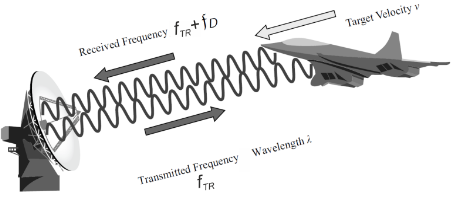
\includegraphics[width=0.6\columnwidth]{../Images/cw.png}
    \caption{Operation of \gls{cw} radar system.}
    \label{fig:cw}
\end{figure}

\gls{cw} \gls{radar} are often used in short-range, low-cost applications \cite{cwradarlecture, pomr} such as the measurement of liquid levels, aircraft detection, short-range navigation, and missile seekers. Manikas states that the use of \gls{cw} \gls{radar} is set to become standard for every new car manufactured, which would possibly make \gls{cw} the most commonly used of any radar variant. \gls{cw} radars use signals across the \gls{rf} \gls{em} spectrum, similarly to pulsed radar. An unfortunate disadvantage of the \gls{cw}, is the reduced dynamic range due to the simultaneous transmission and reception of signals. Because transmission is continuous, it competes with the reflected echoed signal (which is returned as a weaker signal). This can cause the transmitting signal to easily swamp the reflected signal, preventing the detection of targets. However, the Doppler relayed by the moving target is mitigates this effect as the transmitted signal is, effectually, at zero Doppler - this helps to isolate the transmitted and received signals. Separate antennas for transmission and reception are often used to prevent the transmit signal from leaking into the receiving antenna \cite{cwradarlecture, mitlecture}.

Pulsed \gls{radar} differs in that it emits short durations of \gls{em} waves from the transmitter with a defined pulse width, $\tau$ \cite{pomr}. Unlike the \gls{cw} \gls{radar}, the transmitter and receiver are isolated during successive iterations of transmission and reception. When pulses are being transmitted, the receiver is disconnected and no \gls{em} signals are received. Between transmitted pulses, $\tau$, the transmitter is disconnected to allow the receiver to receive reflected \gls{em} signals. A full cycle includes the transmit time of each pulse, $\tau$, and the \emph{"listening"} time by the receiver. This is also known as the \gls{pri}. Figure~\ref{fig:pulsed} illustrates the waveform of a typical pulsed \gls{radar}.

\begin{figure}[htbp]
    \centering
    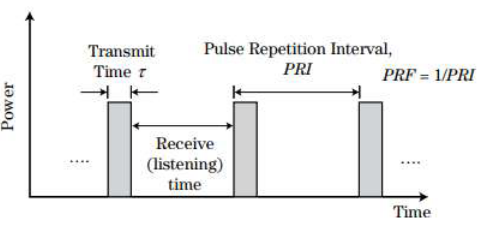
\includegraphics[width=0.6\columnwidth]{../Images/pulsed.png}
    \caption{Typical pulsed \gls{radar} waveform. \cite{pomr}}
    \label{fig:pulsed}
\end{figure}

Reeder et al. in \cite{reeder} signal the difference between pulsed and \gls{cw} \gls{radar} being in their signal aliasing. The pulsed wave Doppler is described as having signal aliasing at high frequencies but with depth acuity, whereas \gls{cw} Doppler is said to have no signal aliasing but does has depth ambiguity \footnote{Depth ambiguity is a concept that recognises that ambiguous figures or images can often be perceived in multiple ways \cite{yu}. A group of figures containing ambiguity in its depth relations can effectually cause either of two surfaces to be seen as being the "front" of an object. There is much research on depth ambiguity resolution which can be explored in \cite{helou} and \cite{blackburn}}. Additionally, \gls{cw} \gls{radar} has rudimentary limitations: range cannot be measured and it produces relatively low \gls{snr} \cite{mitlecture2}. For this matter, large-scale, high-end pulsed \gls{radar} systems are used for improved performance as it has the ability to measure range and Doppler frequency simultaneously. However, pulsed wave Doppler is limited by \gls{prf} - the number  of  transmit/receive  cycles  the  radar completes per second \cite{pomr}, measured in pulses per second (PPS). This requires that the \gls{prf} be low enough so all echoes of interest from a given pulse will return to the radar receiver before the next pulse is transmitted. Equation~\ref{eqn:prf} gives the minimum \gls{prf} that will produce the maximum range of Doppler frequencies that can be measured unambiguously.

\begin{equation}
    PRF_{min} = 2f_{d_{max}} = \frac{4v_{r_{max}}}{\lambda}
    \label{eqn:prf}
\end{equation}

This presents an issue when using pulsed wave Doppler as most modern radars measure the Doppler frequency of the reflected \gls{em} wave; a pulsed \gls{radar} samples the Doppler frequency at the \gls{prf}. If the sampling rate is not high enough, it may lead to Doppler frequency ambiguities. This leads to a conflict between maximising Doppler frequency and lowering \gls{prf} - maximising the unambiguous range leads to lower \gls{prf}, but maximising  the unambiguous Doppler frequency will lead to higher \gls{prf}. This makes \gls{cw} \gls{radar} a more desirable choice as it is not limited by \gls{prf} because the \gls{em} waves are continuously transmitted and received, allowing much higher velocities to be measured.

\section{Processing Radar Data}
Traditionally, a \gls{stft} or spectrogram is used to process radar data from a \gls{cw} radar. A fundamental principle of Fourier analysis is the inverse relationship between time and frequency. Understanding this property and its consequences are a crucial part of understanding Doppler processing techniques.

\subsection{The Short-Time Fourier Transform}
The \gls{stft} is a powerful tool for audio signal processing – it is particularly important for time-frequency distribution analysis \cite{nasser}. The standard Fourier transform (such as the \gls{dft} and \gls{dtft}) takes the average of the frequency information over the signal’s entire time interval. In contrast, the \gls{stft} provides time-localised frequency information. This is useful for situations where the frequency components of a signal vary over time \cite{nasser, smith}. The \gls{stft} only considers a short-duration segment of a longer signal and computes its Fourier transform. This is accomplished by multiplying a longer time function by a window function (commonly-used are the rectangular window and the Hamming window). The window function tapers the longer time signal at the ends of the window function to improve the representation in the frequency domain. The \gls{stft} parameters can be tuned to approximate the time-frequency analysis for spectral display or to measure model parameters in a short-time spectrum. Kehtarnavaz provides the \gls{stft} pair in \cite{nasser}, provided in Equation~\ref{eqn:stft-pair}.

\begin{equation}
    \begin{cases}
        X_{STFT}[m,n]\sum_{k=0}^{L-1}x[k]g[k-m]e^{-j2\pi nk/L}\\
        x[k] = \sum_{m}^{}\sum_{n}^{}X_{STFT}[m,n]g[k-m]e^{-j2\pi nk/L}
    \end{cases}
    \label{eqn:stft-pair}
\end{equation}

Where $x[k]$ represents a signal and $g[k]$ is an $L$-point window function. 

The \gls{stft} of a signal, $x[k]$, can essentially be thought of as the Fourier transform of the product of the signal, $x[k]$, and the shifted $L$-point window function, $g[k-m]$. Figure~\ref{fig:computing-stft} illustrates the computing of the \gls{stft} of a signal, $x(t)$, by taking the Fourier transform of a windowed signal.

\begin{figure}[htbp]
    \centering
    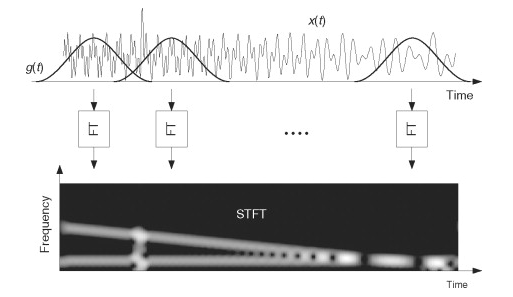
\includegraphics[width=0.6\columnwidth]{../Images/computing_stft.png}
    \caption{Computing the \gls{stft} of signal $x(t)$. \cite{nasser}}
    \label{fig:computing-stft}
\end{figure}

Although effective, there is a trade-off between time and frequency resolution with the \gls{stft} \cite{nasser, smith, pomr}. For example, a narrow-width window provides a better resolution in the time-domain, but results in a poor resolution in the frequency domain. This stands true for a wide-width window except it will then produce better resolution in the time-domain and worse resolution in the frequency-domain. This trade-off is also known as the trade-off between temporal and spectral resolution. The visualization of the \gls{stft} is often realised using its spectrogram, which is essentially an intensity plot of the \gls{stft} magnitude over time. Figure~\ref{fig:tradeoff} illustrates the trade-off made between different time-frequency resolutions.

\begin{figure}[htbp]
    \centering
    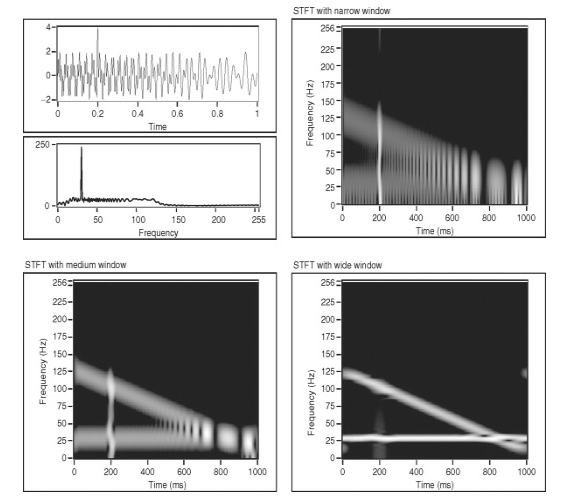
\includegraphics[width=0.6\columnwidth]{../Images/tradeoff.png}
    \caption{Trade-off made between different time-frequency resolutions \cite{nasser}.}
    \label{fig:tradeoff}
\end{figure}


\subsection{The Spectrogram}
The exploration of the \gls{stft} effectively leads to the use of the spectrogram in \gls{radar} signal processing. The spectrogram is a way to visualize the signal strength of a signal over time at various frequencies present in a waveform \cite{yan, griffaton}. In other words, it displays the strength of a signal over time at different frequencies in a waveform. The spectrogram looks at the power of the received signal echoed by the targets – this allows the received power spectrum to detect moving targets. This makes it an ideal tool for radar analysis. This tool is beneficial as it not only illustrates whether there is more or less energy at a particular frequency, but it also does well to represent how the energy levels vary over time. The spectrogram is used in various applications such as in seismology to look at frequency content of continuous wave signals that are recorded by seismometers \cite{yan}. This helps to distinguish and characterize different types of earthquakes and other vibrations in the Earth. Lin makes use of the spectrogram in his Master's dissertation on \emph{Dynamic Hand Gesture Recognition} in \cite{clin}. Figure~\ref{fig:spectrogram-eg} is taken from his dissertation and shows the spectrogram data of a hand waving left and right repeatedly in front of a \gls{radar}. \textsc{MATLAB}'s \textbf{pspectrum} function was used to create this spectrogram with a frequency resolution of 128 Hz. To generate a spectrogram, the \gls{stft} of a time-domain signal is taken and then the \gls{fft} is applied to each short-time division. The spectrogram is then generated as a plot of the spectrum of each segment.

\begin{figure}[htbp]
    \centering
    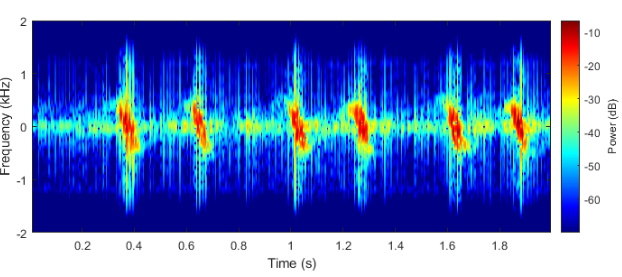
\includegraphics[width=0.6\columnwidth]{../Images/spectrogram_eg.png}
    \caption{Spectrogram data of hand gesture from Lin \cite{lin}.}
    \label{fig:spectrogram-eg}
\end{figure}

\section{Doppler Concepts}
The Doppler \emph{effect} is based on the relative motion between a radar and a target. If this relative motion exists, then the frequency of the reflected \gls{em} wave will be different from the frequency of the wave transmitted by the radar, producing a frequency shift that is proportional to the velocity of the moving target \cite{pomr, ian}. This effect is common to all wave theory and phenomena and is a fundamental principle of wave theory. Equation~\ref{eqn:doppler-shift} gives the equation used to determine the frequency perceived by the radar, relative to the moving target.

\begin{equation}
    f_r = \frac{1+\frac{v}{c}}{1-\frac{v}{c}}f
    \label{eqn:doppler-shift}
\end{equation}

This effect provides interesting possibilities for target detection and speed estimation. An approaching target will cause an increase in the echoed signal received by the \gls{radar}, whereas a target moving away from the \gls{radar} will decrease the received signal \cite{mitlecture2}. This effect is commonly experienced when one is standing near a train or ambulance passing by. The Doppler shift is advantageous in detecting echoes from moving targets which can then be used to determine the range to the target (Equation~\ref{eqn:range}) or the speed of the moving target. This effect is visually represented in Figure~\ref{fig:doppler-shift}.

\begin{figure}[htbp]
    \centering
    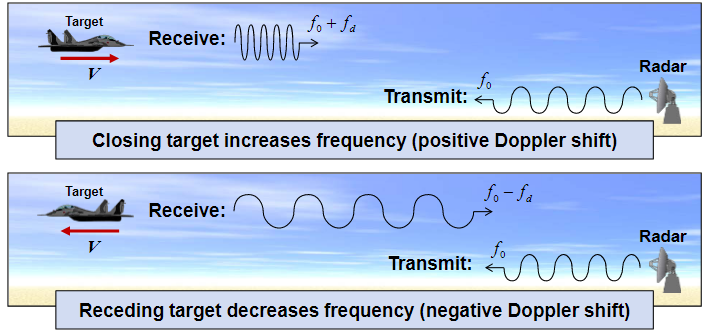
\includegraphics[width=0.6\columnwidth]{../Images/doppler_shift.png}
    \caption{How the Doppler shift works \cite{mitlecture2}}
    \label{fig:doppler-shift}
\end{figure}

This Doppler effect leads to the use of what is called the Doppler \emph{shift}, $f_d$, or Doppler \emph{frequency}. The Doppler \emph{shift} is defined as the difference between the frequency of the respective transmitted and received waves and is approximately given by Equation~\ref{eqn:doppler}.

\begin{equation}
    f_d \approx \frac{2v_r}{\lambda}
    \label{eqn:doppler}
\end{equation}

This equation can be used to determine the speed of the moving target and can be used to express the frequency of the received signal, $f_r$, as a sum of the frequency of the transmitted wave, $f$, and the experienced Doppler shift, $f_d$. This is shown in Equation~\ref{eqn:rec-freq}

\begin{equation}
    f_r = \frac{f}{f_d}
    \label{eqn:rec-freq}
\end{equation}

Notice in Figure~\ref{fig:radial-velocity} that a moving target will produce an angle between the velocity vector of the target and the \gls{radar}'s line-of-sight, $psi$. This introduces the concept of the \emph{radial velocity}. The Doppler shift is proportional to the relative velocity along the line-of-sight between the \gls{radar} and target. Hence, a target viewed at $psi$ = 90 \deg will have a Doppler shift of 0 Hz.

\begin{figure}[htbp]
    \centering
    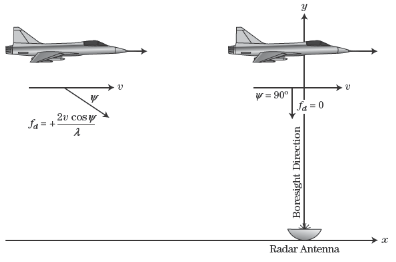
\includegraphics[width=0.6\columnwidth]{../Images/doppler_effect.png}
    \caption{Doppler shift as it relates to radial velocity \cite{pomr}.}
    \label{fig:radial-velocity}
\end{figure}

\section{Existing Vehicle Speed Estimation Implementations}
There have been many implementations of speed estimation devices described in literature, such as the vision-based vehicle speed estimation problem documented in a 2021 academic article by Llorca et al. in \cite{llorca}. There is an increasing necessity to accurately estimate the speed of road vehicles, firstly, because there is a global increasing number of speed cameras installed and, secondly, because traffic monitoring and forecasting plays a vital role in improving traffic and energy consumption in smart cities \cite{llorca}. Vision-based systems are often used for vehicle detection, as their low-cost application does not require expensive range sensors, but they also come with challenges. More recently, vision-based systems have been applied to autonomous vehicles and is still widely used for speed limit enforcement and traffic control and monitoring. The main limitation with vision-based approaches for speed detection is the need for more data than is currently available. Vision-based systems are often operated with machine-learning or deep-learning approaches which require a large amount of data to be able to train complicated models that are able to solve and generalise a general problem from sequences of video input \cite{llorca, montero, wilson}. Montero et al. \cite{motero} and Wilson et al. \cite{wilson} provide more interesting work on the use of a vision-based active safety system for automatic stopping and prevention of road traffic injuries and deaths.

There have been implementations using radar too, such as from Jeng et al. \cite{jeng}. This work was documented in 2014 and uses a 2D range Doppler \gls{fmcw} for estimating the length and speed of a vehicle. A Fourier processor is then used with an \gls{isar} algorithm to extract the range and speed for each vehicle using a single-beam \gls{fmcw}. This work provided accurate measurements using a squint angle with errors of $\pm$4 km/h and $\pm$1 m and was proved to work excellently for small moving targets such as bikes and pedestrians at speeds down to 5 km/h. These range and speed results are shown on 3D spectrum plots in Figure~\ref{fig:jeng}. Although the proposed algorithm exhibited acceptable performance at low speeds there is room to improve the vehicle speed range detection. It is proposed that a \gls{dsp} with higher performance capability could be used to improve the robustness and accuracy of the proposed algorithm.

\begin{figure}[htbp]
    \centering
    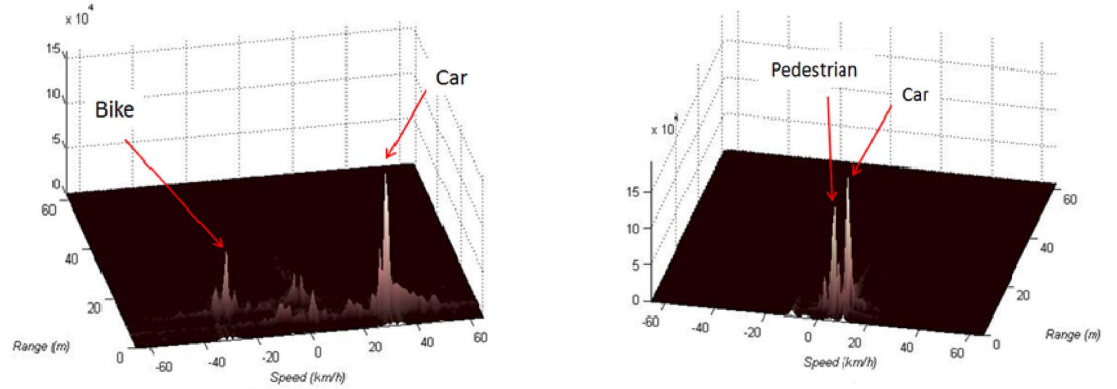
\includegraphics[width=0.6\columnwidth]{../Images/jeng_img.png}
    \caption{Spectrum plot of range and speed of vehicles moving in opposite directions (left) and car and pedestrian moving in the same direction (right)  \cite{jeng}.}
    \label{fig:jeng}
\end{figure}

Further progress on the use of radar for speed estimation has been made using ultrasonic \gls{radar} technology as proposed by Edwards in his thesis report \cite{ian}. Edwards used an ultrasonic and audio radar to determine the speeds of moving sports balls for indoor and outdoor sports training and research purposes. He concluded that audio and ultrasonic radar systems are viable solutions for estimating the speeds of sports balls. Although both the ultrasonic and audio systems performed well for most sport ball sizes indoors within a range of 2.5 m, the audio \gls{radar} system did not perform effectively outdoors. Ultimately, the conclusion was made that ultrasonic \gls{radar} system performed the best, especially with sports balls of a higher \gls{rcs} up to a range of 8.5 m. The speed of sports balls of smaller \gls{rcs} values were not accurately estimated outdoors. Additionally, tests with faster moving sports balls showed lower rates of success with speeds over 10 m/s - this is due to the narrow bandwidth of the ultrasonic transducers used, which limit the maximum observable speeds of the system. Figure~\ref{fig:ian-img} shows a spectrogram result of the ultrasonic and audio radar test for a moving basket ball.

\begin{figure}[htbp]
    \centering
    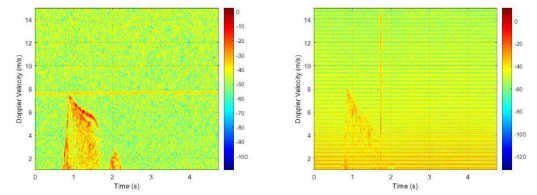
\includegraphics[width=0.6\columnwidth]{../Images/ian_img.png}
    \caption{Spectrogram results for basket ball test using ultrasonic \gls{radar} (left) and audio \gls{radar} (right) \cite{ian}.}
    \label{fig:ian-img}
\end{figure}

\section{Literature Critique}
It is clear from this chapter that a thorough amount of literature exists on the topics of radar, vehicle detection and speed estimation, and the use of \gls{radar} technology in these applications. Much has already been written about the motivations of using \gls{cw} Doppler \gls{radar} over pulsed Doppler and the fundamental use of the spectrogram and \gls{stft} for these applications.

However, in the case of ultrasonic \gls{radar} systems, there lacks a comprehensive amount of research conducted on its use for vehicle speed estimation systems. The literature has established that there is an extensive use of ultrasonic \gls{radar} systems in various industries; it is a trusted and reliable technology especially for low-cost applications. There are existing experimental projects that have explored the use of ultrasonic radar systems for speed detection of objects of interest, but there is a gap in its use for vehicle speed detection. \Gls{rf} systems have traditionally been developed to estimate the speed of a moving vehicle. There has not been sufficient work to develop and fully characterise the performance of an ultrasonic radar system to measure the speed of slow-moving vehicles in a parking area. This report hopes to fill in the gaps omitted by existing ultrasonic \gls{radar} work by documenting the use of ultrasonic \gls{radar} for vehicle speed detection for slow-moving vehicles. Furthermore, the performance of this proposed system will be characterised by its execution in indoor and outdoor parking areas.

% ----------------------------------------------------
\ifstandalone
\bibliography{../Bibliography/References.bib}
\printnoidxglossary[type=\acronymtype,nonumberlist]
\fi
\end{document}
% ----------------------------------------------------